\documentclass[10pt]{siamltex}
\usepackage[]{amsmath,amssymb,epsfig}
\usepackage[top=18mm, bottom=18mm, left=20mm, right=20mm]{geometry}

\usepackage{hyperref}

\usepackage{graphicx}
\usepackage[space]{grffile}

\newcommand{\mb}[1]{\mbox{\boldmath$#1$}}

\usepackage{lineno}

\usepackage{subfigure}
\usepackage{amsmath}
\usepackage{amssymb}
\usepackage{graphicx}
\usepackage{comment}
\usepackage{array}
\usepackage{algorithm}
\usepackage{algorithmic}
\usepackage{url}

\usepackage{setspace}
\usepackage{multicol}
\usepackage{multirow}
\usepackage{color}
\usepackage{colortbl}
\usepackage{xcolor}
\usepackage{hyperref}

\newcommand{\myreferences}{../../../Postdocs_laptop/postdoc_bib_file}

\usepackage{lineno}

\hypersetup{
    colorlinks=true,
    citecolor=red,
    linkcolor=blue,
    urlcolor=blue
  }
  
\usepackage{listings}
\usepackage{color}

\definecolor{dkgreen}{rgb}{0,0.6,0}
\definecolor{gray}{rgb}{0.5,0.5,0.5}
\definecolor{mauve}{rgb}{0.58,0,0.82}

\lstset{frame=tb,
  language=R,
  aboveskip=3mm,
  belowskip=3mm,
  showstringspaces=false,
  columns=flexible,
  basicstyle={\small\ttfamily},
  numbers=none,
  numberstyle=\tiny\color{gray},
  keywordstyle=\color{blue},
  commentstyle=\color{dkgreen},
  stringstyle=\color{mauve},
  breaklines=true,
  breakatwhitespace=true,
  tabsize=3
}

\newcounter{ale}
\newcommand{\abc}{\item[\alph{ale})]\stepcounter{ale}}
\newenvironment{liste}{\begin{itemize}}{\end{itemize}}
\newcommand{\aliste}{\begin{liste} \setcounter{ale}{1}}
\newcommand{\zliste}{\end{liste}}
\newenvironment{abcliste}{\aliste}{\zliste}



\begin{document}

\title{MATH 191 Topics in Data Science: \\ Algorithms and Mathematical Foundations \\ A comparison of correlation measures used for prediction of stock returns }
\author{Lawrence Ouyang}
\date{\today}
\maketitle

\begin{center}
     \today
\end{center}

\vspace{5mm}

\begin{abstract}
The prediction of the returns of a stock has been a very popular problem since the very existence of the stock market. Given the day's returns, what will tomorrow's look like? What will it look like next week, or next month? An idea to examine this is the use of correlation measures. The market is not an isolated system; all things affect one another. This work will use a variety of known correlation measures (Pearson's, Spearman's, Hoeffding, maximal correlation, distance correlation, MIC) to compute the most relevant instruments to which we will apply linear regression. The goal is to find an accurate predictor for future returns. 
\end{abstract}


\begin{keywords} Correlation; Returns; Linear Regression
\end{keywords}


\section{Introduction}

The idea behind examining logarithmic returns is extremely rational. By using returns instead of raw prices, our values become normalized, which is a requirement for accurate comparisons and measurements. Logarithmic functions are log-normal as well, and as such, our returns our now normally distributed. However, with these benefits also come a price. The logarithmic returns does not have an implied one-to-one relationship with the simple returns, as well as having higher variance which can possibly reduce expected returns\cite{CompLogSimRet}. For simplicity, this paper will focus on the use of logarithmic returns to simplify our results.

\subsection{Correlation Measures}

%\vspace{10mm}  % add white space whenever needed

Determining our significant predictors using only a standard correlation measure like Pearson or Spearman would be too mundane. We instead examine other measurements, beginning with the maximal correlation. Maximal correlation 




\begin{figure}[h]
\begin{center}
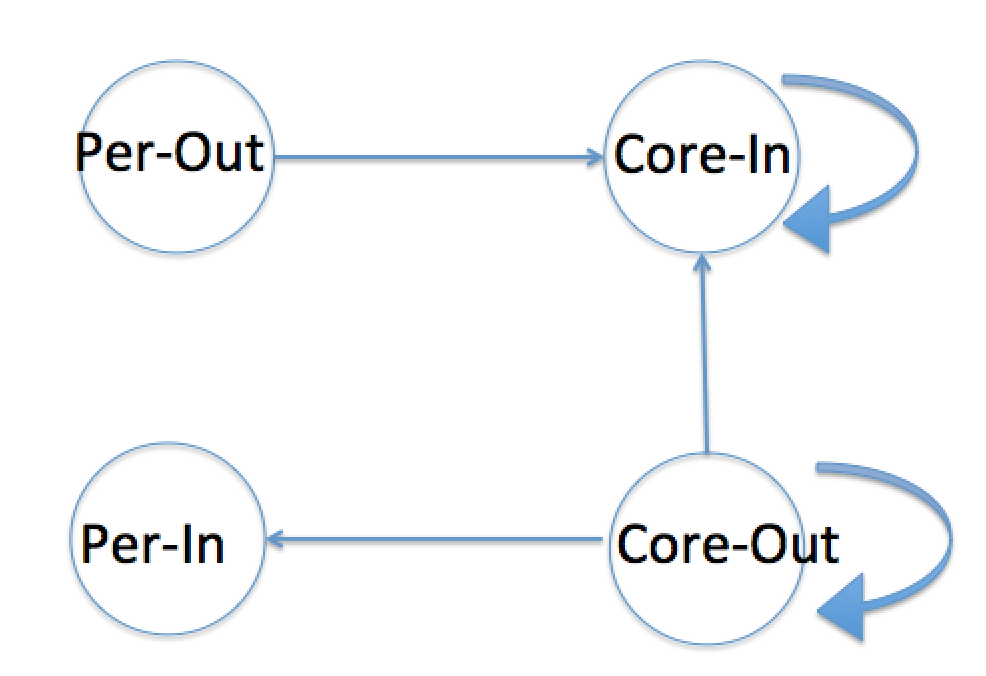
\includegraphics[width=0.46\columnwidth]{Directed_Core_Per}
\end{center}
\caption{This is how you add a plot to a Figure. It is always a good idea to add such a caption to each Figure, and explain what the figure is about. Also, if your plot has x and y axis, please always label your graphs (within MATLAB) so that your plots/results can be easily read and understood.}
\label{fig:DirCorPer}
\end{figure}

In Section \ref{sec:ourWork} we ... 
In Section  \ref{sec:NumExpSyn} we test the above algorithms on synthetically generated data sets, while in Section \ref{sec:NumExpReal} we do so for a real data set. Finally, in Section  \ref{sec:conclusion} we conclude with a summary of our results, and discuss future possible research direction. 



\section{Related work} \label{sec:relWork}

\textbf{Questions/Comments/Things that could be done}
\begin{itemize}
\item What is a good notion of core-periphery structure in directed networks? Would the null model shown in Figure \ref{fig:DirCorPer} be a good model?
\item Can one build on or expand some of the above methods and apply them to directed networks? 
\item As a starting point, perhaps apply simulated annealing to the objective function induced by the above null model
\item Apply this to a real network, a good such example might be the migration network between counties in the United States, which we have seen in class in the past.
\item This is how you add an url link 
 \begin{center}
   \url{http://people.maths.ox.ac.uk/porterm/papers/prestige_final.pdf} 
\end{center}   
\end{itemize}

\textcolor{red}{This is how you color tex in red ...}

\textcolor{blue}{This is how you color tex in blue ...}

\section{Our work}    \label{sec:ourWork}
\subsection{The Data}

The data set being used is the logarithmic return prices from date to date for 477 stocks. Since the data contains many not-available entries, we begin by stripping those out of our measurements. Instruments with a high number of NA entries are entirely removed along with missing rows. This leaves us with a dataset containing number instruments with data for number of days.

\subsection{The Process}
With our primmed and proper data, we begin by calculating their coefficient matrices. Considering the size of our data, the calculation of our coefficient matrices take a very large amount of time. Consider the following R code to compute the correlation coefficients:
\begin{lstlisting}
# Consider the given RETS matrix, remove poor columns and rows:

RETS = na.omit(RETS);
numStock = dim(RETS)[2];

# Calculate the various correlations:
# Pearson, Spearman:
PCOR = cor(RETS, method = "pearson");
SCOR = cor(RETS, method = "spearman");

#Maximal
#install.packages('acepack');
MaxCOR = matrix(, nrow = numStock, ncol = numStock);
colnames(MaxCOR) = colnames(RETS);
rownames(MaxCOR) = colnames(RETS);

for (i in 1:numStock) {
	for(j in 1:numStock) {
		transfVars = ace(RETS[,i],RETS[,j]);
		MaxCOR[i,j] = cor(transfVars$tx,transfVars$ty)[1];
	}
}

#Hoeffding's D
#install.packages('Hmisc');
HCOR = hoeffd(RETS)$D;

#Distance
DCOR = matrix(, nrow = numStock, ncol = numStock);
colnames(DCOR) = colnames(RETS);
rownames(DCOR) = colnames(RETS);
#install.packages('energy');
for (i in 1:numStock) {
	for(j in 1:numStock) {
		DCOR[i,j] = dcor(RETS[,i],RETS[,j]);
	}	
}

#MIC
#install.packages('minerva');
MICCOR = mine(RETS,n.cores = 4)$MIC
\end{lstlisting}
Of course, this is the simple part. Now for the instrument we would like to predict, we need to sort it's correlation values in descending order, and choose the amount to use in our linear regression. Once sorted, we build our linear regression model and evaluate its accuracy. 
\section{Numerical experiments on synthetic data}  \label{sec:NumExpSyn}
Present here the numerical results you obtain on a synthetically generated data set...

\section{Numerical experiments on real data}   \label{sec:NumExpReal}
Present here the numerical results you obtain on a real data set...


\section{Summary and conclusion}  \label{sec:conclusion}
Summarize your work in this section.


\bibliographystyle{siam}
\bibliography{project_math191}

\end{document}



